% This is samplepaper.tex, a sample chapter demonstrating the
% LLNCS macro package for Springer Computer Science proceedings;
% Version 2.20 of 2017/10/04
%
\documentclass[runningheads]{llncs}
%
\usepackage{graphicx}
\usepackage{listings}
\usepackage[T1]{fontenc}
\usepackage[portuguese]{babel}
\usepackage{hyphenat}
\hyphenation{mate-mática recu-perar}
\usepackage{xcolor}
\usepackage{amsmath}
\usepackage{hyperref}
\usepackage{wrapfig}

\definecolor{codegreen}{rgb}{0,0.6,0}
\definecolor{codegray}{rgb}{0.5,0.5,0.5}
\definecolor{codepurple}{rgb}{0.58,0,0.82}
\definecolor{backcolour}{rgb}{0.95,0.95,0.92}

\lstdefinestyle{mystyle}{
    backgroundcolor=\color{backcolour},   
    commentstyle=\color{codegreen},
    keywordstyle=\color{magenta},
    numberstyle=\tiny\color{codegray},
    stringstyle=\color{codepurple},
    basicstyle=\ttfamily\footnotesize,
    breakatwhitespace=false,         
    breaklines=true,                 
    captionpos=b,                    
    keepspaces=true,                 
    numbers=left,                    
    numbersep=5pt,                  
    showspaces=false,                
    showstringspaces=false,
    showtabs=false,                  
    tabsize=2
}

\lstset{style=mystyle}




\begin{document}
%

\begin{titlepage}
   \begin{center}
       \vspace*{1cm}

       \textbf{Theoretical project 1}

       \vspace{0.5cm}
        Theoretical project 1,   Mobile Robotics
            
       \vspace{1.5cm}

       \textbf{José António Filipe Santos, 98279} 
       \vfill

            
       \vspace{0.8cm}
     
       
\includegraphics[width=0.4\textwidth]{logo.jpg}
            
       Departamento de Electrónica, Telecomunicações e Informática\\
        Universidade de Aveiro\\
       Portugal\\
       May, 2023


            
   \end{center}
\end{titlepage}



\title{Theoretical project 1}
\begin{abstract}
Creation of a Extended Kalman Filter for application in a mobile robot in Matlab.
\keywords{Mobile Robotcis \and Extended Kalman Filter}
\end{abstract}
%
%
%
\section{Introduction}
This work is made with the objective of a virtual robot in an environment with multiple landmarks is 
able to localize itself using an Extended Kalman Filter. The robot is able to locate itslef in this environment 
thanks to the BeaconDetection() function. The other important function is the EKF or Exetended Kalman Filter,
with was modified to meet the requirements of the teacher.





\section{functions}
In this part of the report i will explain the functions that were created and a brief explanation of how they work.


\subsection*{Plotting\_path}
This function has two objectives, one obtainin the steps needed to reach the goal, passing through the landmarks 
and the other is to use the function in Matlab named \textbf{pchip()} to obtain the smooth path that the robot will take.

For the calculation of steps, this is based on the distance between beacons, or between the initial position and the first beacon.

\begin{wrapfigure}{r}{0.5\textwidth}
    \centering
    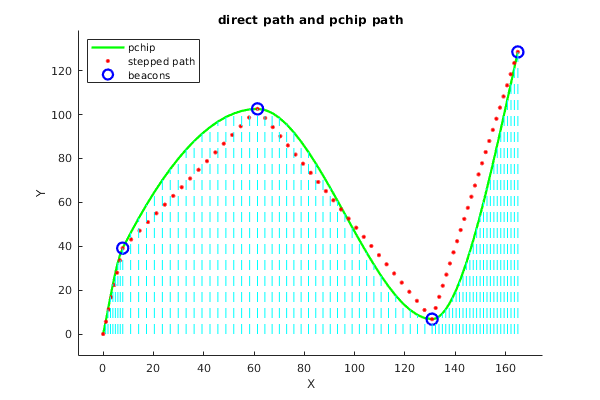
\includegraphics[width=0.48\textwidth]{plotting_path.png}
    \caption{Plotting\_path function results}
    \label{plotting_path_fig}
\end{wrapfigure}

The equation \begin{math} \left(\frac{\sqrt{((x2-x1)^2+(y2-y1)^2}}{\mathrm{Dt}\, * \mathrm{Vn}}\right)
\end{math} is used to obtain the number of steps taken between beacons, where the time step and velocity.
With the number of steps aquired, we can obtain the total number of  points, each with x and y variables.
\\ 
After obtaining the total x and y values evenly spaced between the beacons, we use the \textbf{unique()} function to obtain the unique x values, 
and with these interpolated values or "xintep" values, we use the pchip function to obtain the interpolated y values,these being plotted with all the beacons and evenly spaced points.
The results of this function the figure \ref*{plotting_path_fig}, is showed on the right. 

\break


\subsection*{Plotting\_velocities}

\begin{wrapfigure}{r}{0.5\textwidth}
    \centering
    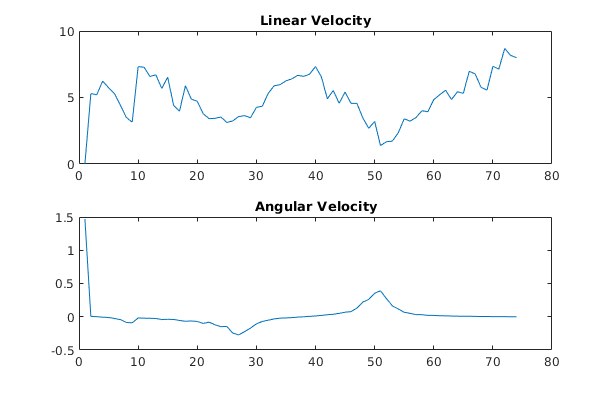
\includegraphics[width=0.43\textwidth]{plotting_velocities.png}
    \caption{Plotting\_path function results}
    \label{plotting_vel_fig}
\end{wrapfigure}

This function uses the \textbf{pchip()} interpolated coordinates to obtain the velocities of the robot. 
To calculate the linear and angular velocities we will use to generate the values for the Extended Kalman Filter, we use the following equations:
\\
\begin{math}
    distance=\sqrt{(x2-x1)^2+(y2-y1)^2} \\  \theta=\sin(y2-y1)/distance
\end{math}
\\
The velocity noises for the velocity are calculated by multiplying noise variable with a random sample from a standard normal distribution.

The caltulations for the linear and angular velocities are:
\begin{center}    
    \begin{math}
        \mathrm{Vn}=\frac{distance*(1+noise)}{\mathrm{Dt}} \ \ ; \ \ \mathrm{Vt}=\frac{\theta*(1+noise)}{\mathrm{Dt}}
    \end{math}.
\end{center}




\subsection*{Generate\_ekf\_data}
This function is used to generate the main data that will be used on the Extended Kalman Filter. 
Most of this variables are used to assist the prediction, such as \textbf{control\_imput\_mea} and \textbf{obs\_range\_bearing}, 
while others are used to verify the accuracy of the Extended Kalman Filter,for example  \textbf{xstate\_true,} and \textbf{control\_imput\_true}.  
In this function other variables were made, mostly for ease of creating other functions, these being \textbf{landmarkxy,} and \textbf{obs\_landmark\_ID}.

\subsection*{ekf\_calculations}
This function is used to prepare the values used in the extended Kalman Filter. Due to most of the variables having information about all states, its needed to obtain the true and estimated position, control input and the range and bearing of the beacons at that time.\\
After this, the function \textbf{ekf} will calculate the estimated position of the robot and with this we can see the estiamtions of the robot, by comparing it to the true values of the robot, these being in the variable \textbf{xstate\_true}.
\\The image \ref*{ekf_calculations_fig} ,listed below shows the result of the \textbf{ekf\_calculations} function, showing in red the true values and in blue the estimated values calculated by the Extended Kalman Filter.

\begin{figure}
    \centering
    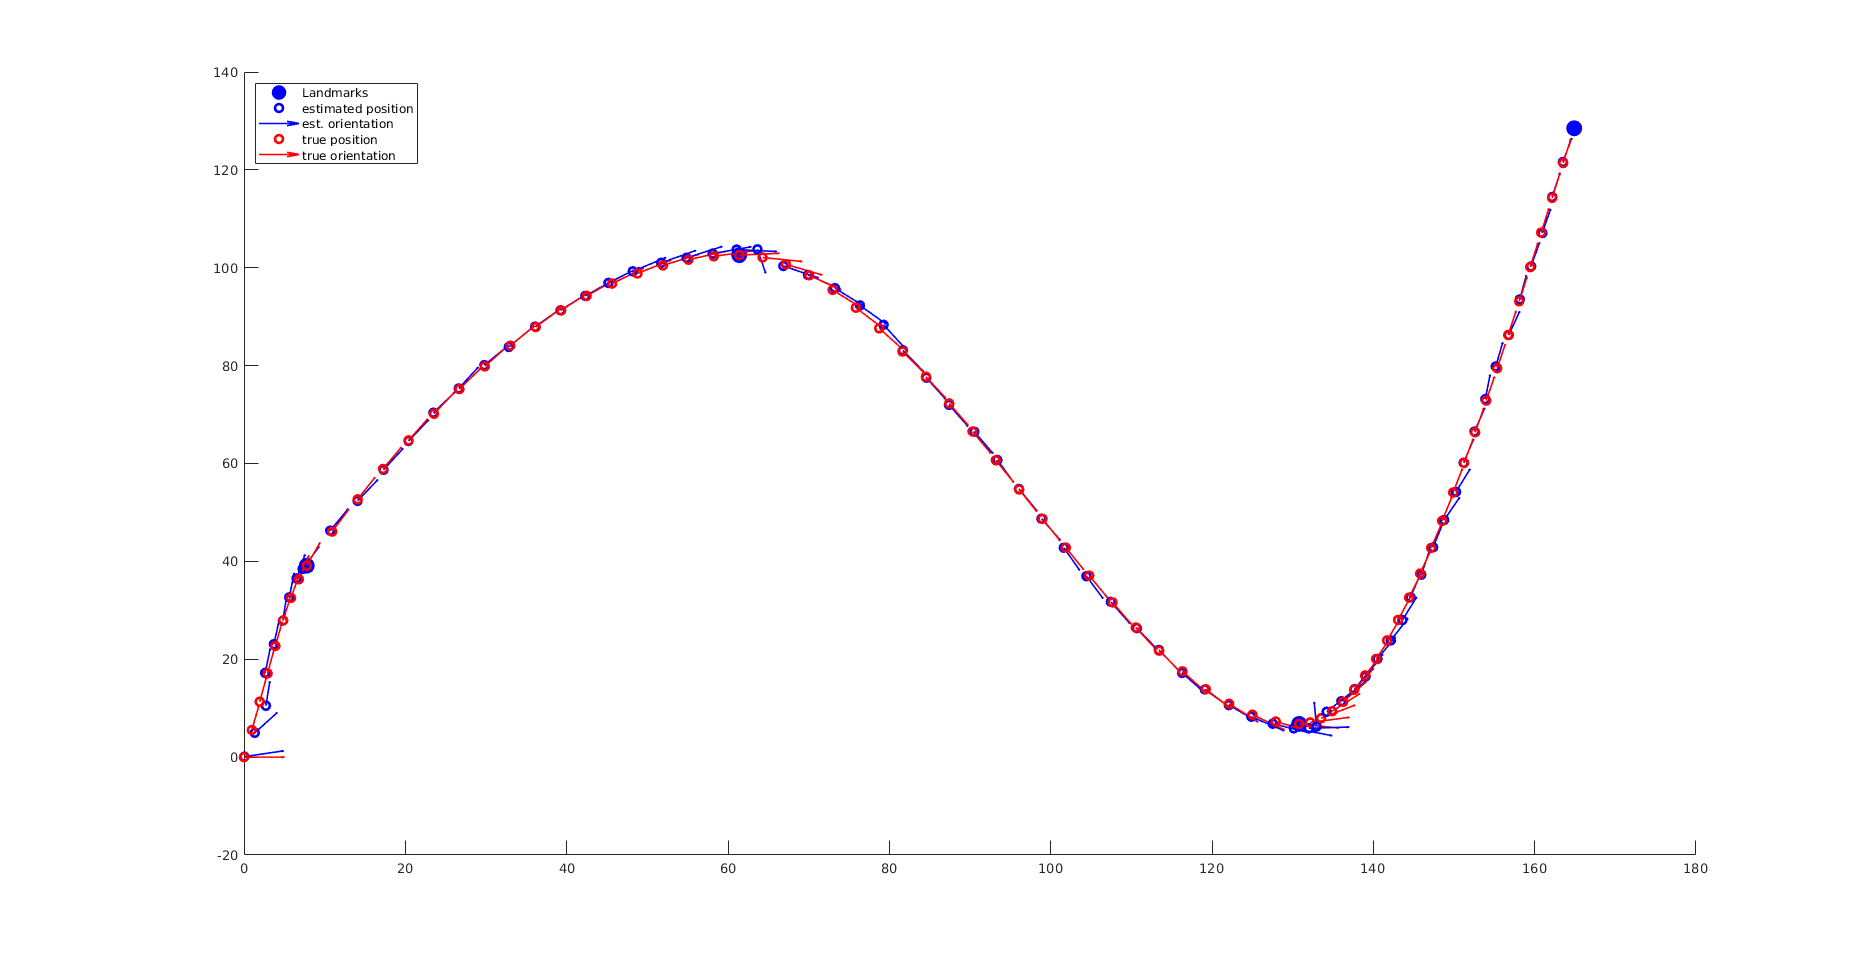
\includegraphics[width=\textwidth]{ekf_calculationspng.png}
    \caption{ekf\_calculations function results}
    \label{ekf_calculations_fig}
\end{figure}


From this image we can see that the estimated values are very close to the true values,
however the estimations orientation when passing the beacons is not as accurate as the positions further away from the beacons.
To be able to see more clearly the errors, the table \ref{errors table}  was made to be able to see the average,largest, smallest errors, and the standard deviation of the errors.
\begin{table}[h]
    \centering
    \caption{Errors for x, y, and theta values}
    \label{errors table}
    \begin{tabular}{|l|l|l|l|l|}
    \hline
    & Average error & Smallest error & Maximum error & deviation \\ \hline
    $x$ & 0.200152 & 0.000000 & 0.754331  & 0.159424 \\ \hline
    $y$ & 0.274439 & 0.000000 & 1.852798 & 0.331390  \\ \hline
    $\theta$ & 0.079925 & 0.000000 & 1.160790 & 0.175788 \\\hline
    \end{tabular}
    \end{table}



\subsection*{EKF}
This function is used to calculate a estimated position and orientation of the robot. 


The first step is calculating the  initial estimation of the robot. 
This is made by using the function \textbf{motionmodel(xstate,Vin,Dt,t)}\\
\begin{math}
    x_{\text{state}} = x_{\text{state}} + (V_{\text{in}}(1) + D_n(1))t\cos(theta_{\text{state}}); \\
    y_{\text{state}} = y_{\text{state}} + (V_{\text{in}}(1) + D_n(1))t\sin(theta_{\text{state}}); \\
    theta_{\text{state}} = theta_{\text{state}} + (V_{\text{in}}(2) + D_n(2))t
\end{math}

This function estimates the x,y and orientation on the step being estimated on the EKF. 
\\ \\
The next step is to calculate the uncertainty of the robot, this is done by calculating the matrix of the predicted covariance,or uncertainty, and noise.
The uncertainty Matrix is calculated by the following equations: 
\begin{center}

\begin{math}
    \text{Jfx}=
    \begin{bmatrix} 
        1 & 0 & -\delta_t\cdot\text{controlinput}\cdot\sin(\text{est}_\theta) \\
        0 & 1 & -\delta_t\cdot\text{controlinput}\cdot\cos(\text{est}_\theta) \\
        0 & 0 & 1
    \end{bmatrix}
\end{math}

\begin{math}
    \text{Jfw}=
    \begin{bmatrix}
        \delta_t\cdot\text{controlinput}\cdot\cos(\text{est}_\theta) &0 \\
        \delta_t\cdot\text{controlinput}\cdot\sin(\text{est}_\theta) &0 \\
        0 & \delta_t
    \end{bmatrix}
\end{math}

%uncertainty calculation 
\begin{equation}
    \text{uncertainty} =\text{Jfx}\cdot P_t \cdot \text{Jfx'}+\text{Jfw}\cdot Q \cdot \text{Jfw'}  
\end{equation}

\end{center}

The next step is to use the \textbf{sensormodel(xym,xstate1,ndnphi)}function to get a predicted range and bearing with noise from the position(xstate1) of the robot. 
\\\begin{math}
    bearing=\sqrt{(x-xstate)^2+(y-ystate)^2}+\text{ndnphi} \\
    angle=\arctan2(y-ystate,x-xstate)-\theta+\text{ndnphi}
\end{math}
\\
With the predicted range and bearing we can subtract both of them and obtain the error,this being the variable \textbf{innov} that will be used for the calculations later.
\\

Another calculation step is to obtain the Jacobian of the sensor model, this is done by follwoing these equations:
\
\begin{equation}
a = \frac{x - xym(1)}{\sqrt{(x - xym(1))^2 + (y - xym(2))^2}}, \quad
b = \frac{y - xym(2)}{\sqrt{(x - xym(1))^2 + (y - xym(2))^2}}, \\ \quad 
c = 0;
\end{equation}

\begin{equation}
d = -\frac{(y - xym(2))}{\left(\frac{(y - xym(2))^2}{(x - xym(1))^2} + 1\right)(x - xym(1))^2}, \quad
e = \frac{1}{\left(\frac{(y - xym(2))^2}{(x - xym(1))^2} + 1\right)(x - xym(1))}, \\ \quad
f = -1;
\end{equation}

\begin{equation}
J = \begin{bmatrix}
a & b & c \\
d & e & f
\end{bmatrix}
\end{equation}
The final jacobian matrix  will be used in the next step, this being the Kalman Gain.

One of the last steps of the Extended Kalman Filter is to calculate the Kalman Gain and the new estimated position and orientation of the robot.
In the equations below, we calculate \textbf{S}, the measurement error covariance and \textbf{K}, the Kalman Gain.\\

\begin{center}
    
    \begin{math} 
        S=J\cdot P_t \cdot J'+R \quad ; \quad K=P_t \cdot J' \cdot S^{-1}
    \end{math}
\end{center}
    
The final step of the EKF is to calculate the new estimated position and orientation of the robot, this is done by the following equations:
\\ 
\begin{center}
\begin{math}
    x_{t+1}=x_t+K\cdot(innov) \quad ; \quad P_{t+1}=(I-K\cdot J)\cdot P_t
\end{math}
\end{center}

\subsection*{plotting\_robot\_atributes}
In this function, we calculate and plot the values requested by the teacher, regarding the virtual use of the Direct Drive robot and the Tricicle robot. 
The results of these equations are below, where we can see the slight variations between the left and right Direct Drive robot, and the similarities between those and the Tricicle robots' rear velocity.

\begin{figure}
    \centering
    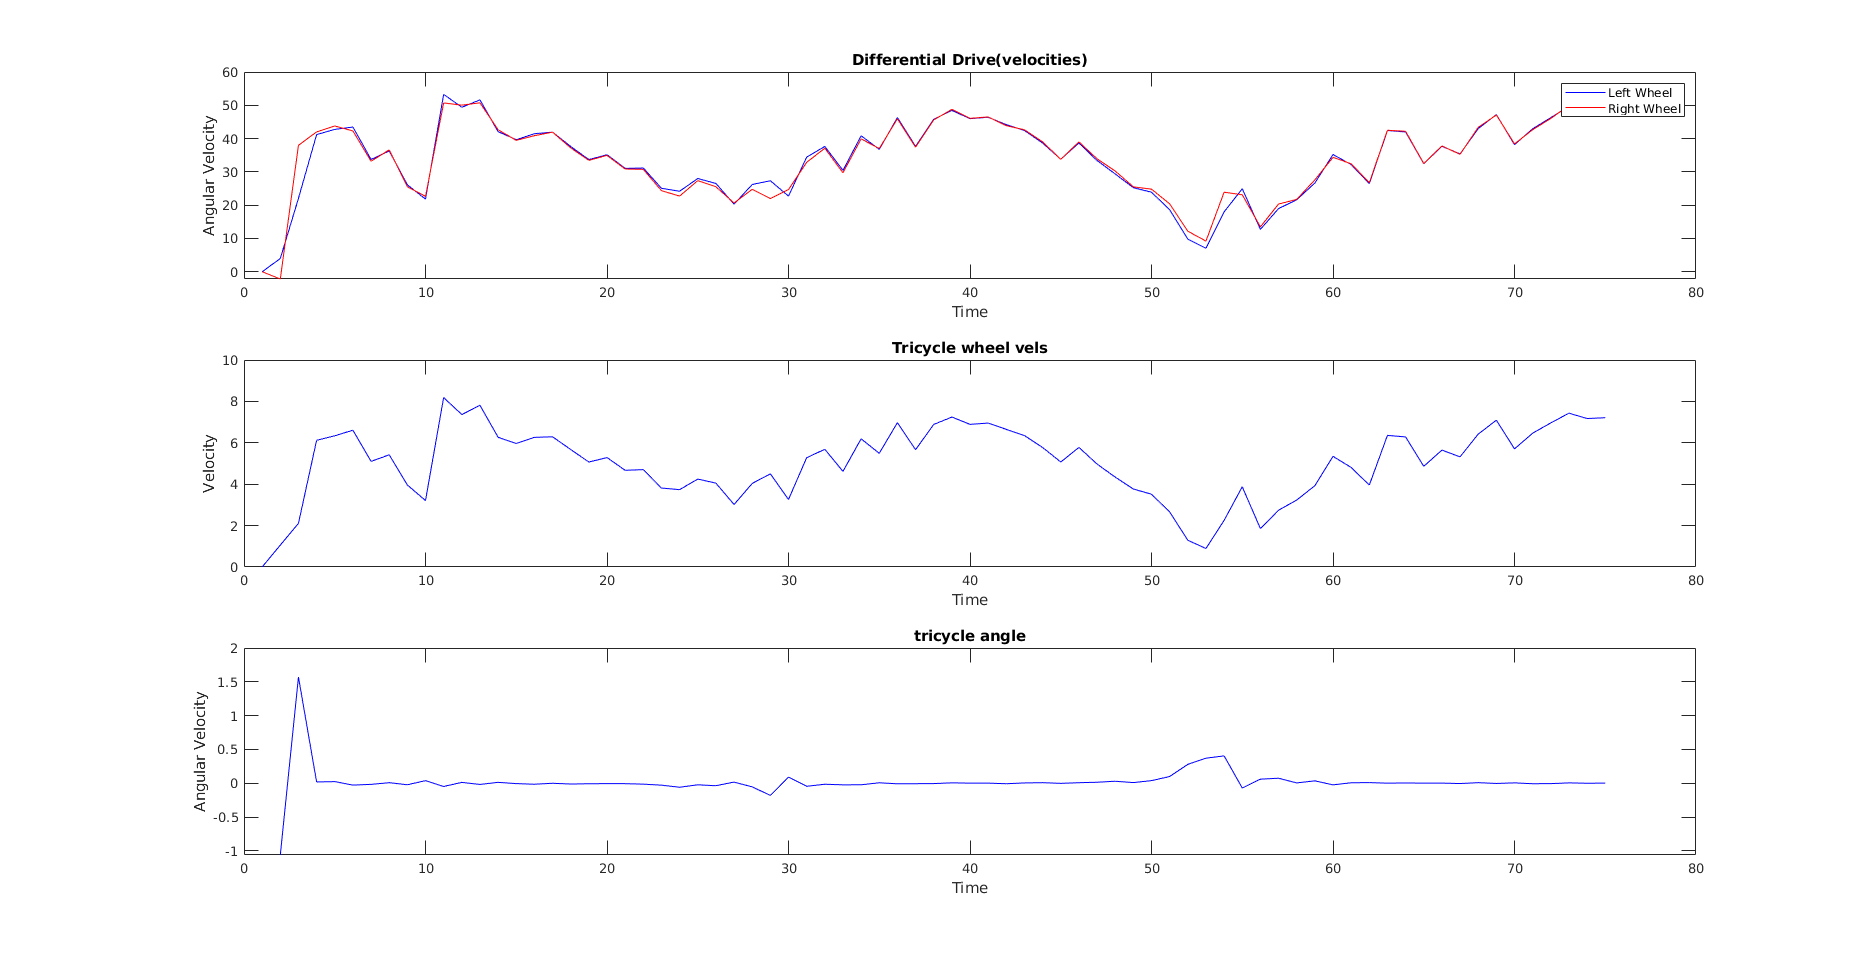
\includegraphics[width=\textwidth]{plotting_robot_vels.png}
    \caption{Plotting\_path function results}
    \label{plotting_robot_fig}
\end{figure}




\subsubsection*{Direct Drive Robot}
The calculations for the Direct Drive velocities are based on the equations of the classes. The equations are the following:
\\
\begin{center}
    
    \begin{math}
        \text{DD}_{left} = \frac{v - w\frac{L}{2}} {r}; \quad
        \text{DD}_{right} = \frac{v + w\frac{L}{2}} {r}
    \end{math}
\end{center}

\subsubsection*{Tricicle Robot}
The calculations for the Tricicle velocities are based on the equations of the classes. These were the equations used:

\begin{center}
    
\begin{math}
    \text{TRI}_{velocity} = v - w \cdot L ;\quad
    TRI_{\alpha} = \arcsin(\frac{w \cdot L}{  \text{TRI}_{velocity}})
\end{math}
\end{center}


\section{conclusion}


In conclusion, this project was a great way to understand the concepts of the
Extended Kalman Filter and how to use it in a practical way. EKF is a very good system that predicts the position of a robot, but it is not perfect, as we can
see in the results, the estimated path is not the same as the real path, this is
because of the noise of the sensors and the noise of the robot’s movement, which
is not taken into account.
\\ This is a very good way to estimate the
position of the robot, but it is not perfect as it has it's limitations.
The results of the Direct Drive and the Tricicle robots are very similar because the equations used to calculate the velocities are very similar being the only difference it's length of the Tricicle robot as well as the third wheel


\end{document}